%%%%%%%%%%%%%%%%%%%%%%%%%%%%%%%%%%%%%%%%%%%%%%%%%%%%%%%%%%%%%%%%%%% 
%                                                                 %
%                            CHAPTER FOUR                        %
%                                                                 %
%%%%%%%%%%%%%%%%%%%%%%%%%%%%%%%%%%%%%%%%%%%%%%%%%%%%%%%%%%%%%%%%%%% 
 
\chapter{Numerical Test Problems}

In this section, we use three numerical experiments to verify and investigate
the proposed algorithms.  The first experiment explores the ability of the
optimization algorithm to handle a nonconvex objective.  The second
experiment investigates the scalability of the predictor-corrector algorithm
using the approximate SVD preconditioner and compares the performance against a
state-of-the-art active-set optimization library.  Finally, the third experiment
exercises the algorithms on a difficult structural sizing problem. 
  
\padd{In all the test problems, the convergence plots show the change of relative
optimality and feasibility along with the optimization iteration. The optimality 
measures the norm of the first two row blocks in \eqref{eq:opt00x}, while the norm of the
last row blocks measures the feasibility. For simplicity, the convergence plot only shows 
the predictor points before $\mu$ reaches zero, plus all the corrector points at $\mu$ equals zero.
Default parameters adopted for all the tests, together with a recommended range, and parameters used 
for generating the results here are listed in Table \ref{tab:param} }

\begin{table}[tbp]
  \begin{center}
    \caption{Parameters used in the test problems \label{tab:param}}
    \setlength\tabcolsep{1.5pt}
  \begin{tabular}{ l c c c c c}
    \textbf{Parameters} & $\textbf{Default}$  & $\textbf{Range}$ & $\textbf{Nonconvex}$ & $ \textbf{Quadratic} $ & \textbf{Structural}  \\ \hline
    \multicolumn{6}{ l }{Predictor-Corrector Algorithm} \\    
    \hline
    $K_{\max}$             	&  100     & $\geq$100         & 100 	 &  100       &    100     \\ 
    $\tau_{\text{opt}}$	           		&  1e-6     & [1e-8, 1e-3]   & 1e-7 	 & 1e-7       &    1e-4    \\ 
    $J_{\max}$  		&   2         & $\geq$2         & 2             & 2           &      2        \\
    $\epsilon_F$    		&   0.1      & [0.1,0.5]	        & 0.1          & 0.1	 &     0.1    \\
    $\epsilon_H$    		&   0.1      & [0.1,0.5]	        & 0.1          & 0.1	 &     0.1    \\
    \textbf{$\alpha_0$}             &  0.05     & $\geq$0.01         & 0.05	 & [40,60,80,100,120]  &  0.05  \\
    $\delta_{\text{targ}}$      &  1.0	& [1.0,10]          & 20		 & 10    &   1.0    \\
    $\phi_{\text{targ}}$   & 10.0	& [5.0,50] 	       & 10		 & 20    &   10     \\
    $\zeta_{\max}$ 		        &  50		& [10,50]	       & 50		 & 50    	 &   50     \\
    $\zeta_{\min}$ 		        &  0.5	& 0.5		       & 0.001	 & 0.001    &   0.5   \\
    $\Delta \mu_{\max}$		        &  -5e-4	& [-5e-4, -5e-1]  & -5e-4	 & -5e-4     &  -5e-4  \\  
    $\Delta \mu_{\min}$		        &  -0.9	& -0.9 	       & -0.9		 & -0.9       &  -0.9    \\
    Fraction Rule    &  True     & True, False    & False	 & False     &   True   \\
    \hline
    \multicolumn{6}{ l }{Preconditioner} \\ 
    \hline    
    $\mathbf{{n_{\mat{\Sigma}}}}$    & 5	       & $\geq$2		& 5	         &  5          &  [20,80,320]  \\
    $\beta$				& 1.0	       & [0.01, 10]        & 1.0         &  1.0       &  0.1  \\
    $N_{\text{bfgs}}$		& 10	       & [1,  20]		& 10 		 &  10	& 10  \\
   $c_{\min}$				& -1	       & [1e-3 1e-1]	& 1e-3	 &  1e-3	& -1  \\
    $\mu_e$			& -1	       & [ -1 , 1] 		& -1.0	 &  -1	& 1e-3  \\
    $\Sigma_e$			& 1 	      & [0,1]                 & 1		& 1		& 1e-3  \\
    \hline
    \multicolumn{6}{ l }{Krylov Iterative Solver} \\ 
    \hline       
    $n_k$		& 20        & [10,30]              & 20		 &  20       &  20  \\
    $\tau_{\text{krylov}}$	& 1e-2     & [0,0.1]           	&1e-2	 &  1e-2    &  1e-4  \\
    \hline
  \end{tabular}
  \end{center}
\end{table}

\section{Non-convex Problem}

We consider the following simple nonconvex optimization problem:
\begin{equation*}
\begin{aligned}
&\underset{x \in R^{100}} {\text{min}}  
& &\phantom{-} \frac{1}{2}x^T \mat{Q} x \\
  & {\text{subject to}}
& &-1 \leq x_i \leq 1 \qquad \forall i = 1,2,\ldots,100 \\
\end{aligned}
\end{equation*}
where $\mat{Q} = \textsf{diag}(1,-1,1,\ldots,1,-1)$ is randomly generated.  The objective is
separable, so it is easy to see that the local minimizers are given by
\begin{equation*}
  x^{*} = \begin{bmatrix} 0 & \pm 1 & 0 & \cdots & 0 & \pm 1 \end{bmatrix}^{T}.
\end{equation*}

This problem is challenging for Newton-based optimization algorithms, because it
has many stationary points that satisfy $F(q) = 0$ but are not local
minimizers. For example, the origin $x=0$ is a local maximizer when $\mat{Q}_{ii} = -1$ .
In addition, when $\mat{Q}_{ii} = 1$, the upper and lower bound $x = \pm 1$ are also 
stationery points where the gradient of the Lagrangian is zero. 

\padd{We ran the optimization algorithm on a set of 1000 random cases. For each case, 
the distribution of $1$ and $-1$ in $\mat{Q}$ is uniformly randomly generated; 
 the initial point $x_0$ is also generated with uniform probability from $\Omega = \{ x \in \mathbb{R}^{100} \; |
\; -2 \leq x_i \leq 2 \}$ in the optimization.  Figure~\ref{fig:nonconvex} shows the 
statistical performance of the optimization algorithm in bypassing stationery points with infeasible starting
points. In $69\%$ of the times, or 
$690$ out of the total $1000$ cases, the algorithm successfully located all the local minimizers. 
In $0.3\%$ of the time, or $3$ out of $1000$ cases, the algorithm converged to $4$ stationery points
with the rest $96$ local minimizers successfully recovered. Overall, an average of $0.41$ stationery points
from the $100$ separable quadratic problems with a Standard Deviation of $0.70$ are delivered by the algorithm. }

\padd{A typical convergence plot from the nonconvex study is provided in Figure~\ref{fig:nc_converg}. Figure~\ref{fig:ncmu} shows the
change of optimality and feasibility at each Homotopy iteration of different $\mu$. Note that for simplicity, 
only the Predictor points are displayed when $\mu > 0$, while the Corrector points are displayed at $\mu = 0$.
Figure~\ref{fig:nccpu} shows convergence 
plot in CPU time, which is used more later when the results are compared with other optimization package. }

\padd{The results show that the optimization method can start from infeasible points, and can handle certain amount 
of nonconvexity. The preconditioner is not used here. }

\begin{figure}[tbp]
  \centering
  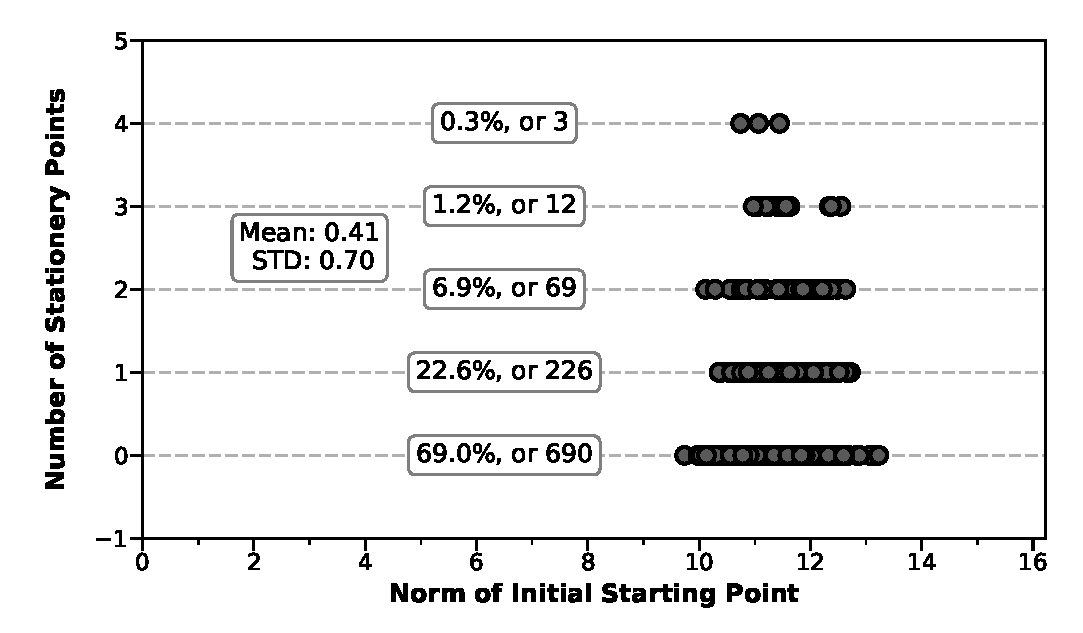
\includegraphics[clip,width=0.7\columnwidth]{./figs/newres2/1000_random.eps}%
  \caption{Stationery Points Distribution. \label{fig:nonconvex}}
\end{figure}

\begin{figure}[tbp]
   \centering
    \subfloat[Convergence vs. $\mu$ \label{fig:ncmu} ]{ 
     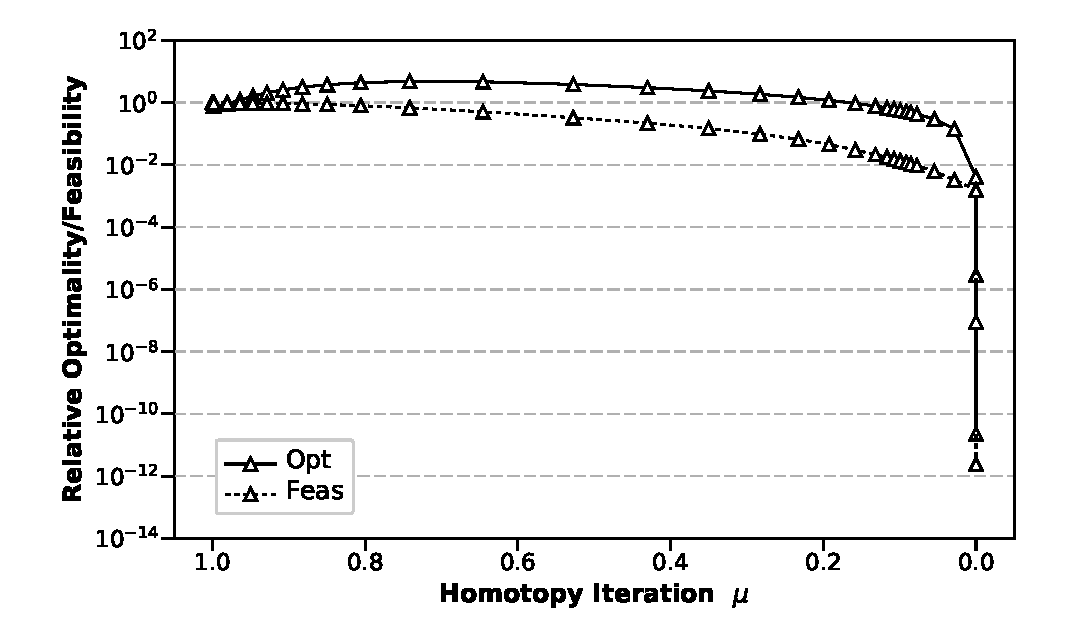
\includegraphics[width=0.7\textwidth]{./figs/newres2/1000_random_mu.eps} } 
     \hspace{1em}
     \subfloat[Convergence vs. CPU time \label{fig:nccpu}]{
     \includegraphics[width=0.7\textwidth]{./figs/newres2/1000_random_cpu.eps} }
    \caption{Typical Convergence Plots in $1000$ Random Cases \label{fig:nc_converg}}
\end{figure}

\begin{remark}
  The parameters $\alpha_0$, $\delta_{\text{targ}}$, $\phi_{\text{targ}}$, and
  $\Delta \mu_{\max}$ all play a role in the ability of Algorithm~\ref{alg:pc}
  to handle nonconvex objectives.  If these parameters are set too agressively,
  then the algorithm may move off the homotopy level-set and converge to a local
  maximizer or saddle, even for the simple problem considered here.
\end{remark}

\section{Scalable quadratic optimization problem}

The next numerical experiement is intended to test the approximate SVD
preconditioner defined in Algorithm~\ref{alg:precond}.  In particular, we are
interested in how this algorithm performs as the number of design variables
increases.  To this end, we consider the following scalable optimization problem
in which we can independently control the size and conditioning of the Hessian
and constraint Jacobian:
\begin{equation*}
  \begin{aligned}
    &\underset{x \in R^n} {\text{min}}  
    & & \frac{1}{2}x^T \mat{Q} x + g^T x \\
    &\text{subject to} & & \mat{A}x \geq b  \\
  \end{aligned}.
\end{equation*}
\padd { The vectors $g\in \mathbb{R}^{n}$ are randomly sampled from a uniform distribution 
in $[ 0,1)$, while $b \in \mathbb{R}^{n}$ from $[0,0.1)$ }

The Hessian $\mat{Q}$ is diagonal with entries
\begin{equation*}
  \mat{Q}_{ii} = \begin{cases}
    \frac{1}{i}, &  i = 1, 2, ...,  \kappa, \\
    \frac{1}{\kappa}, & i = \kappa,  \kappa+1, ... , n, \\
  \end{cases}
\end{equation*}
where $\kappa \leq n$.  This definition produces a Hessian with a condition
number of $\kappa$. \padd{This definition produces a Hessian whose condition number
stays the same as the dimension of the problem increases from $100$ to $500$. }

\padd{
The constraint Jacobian $\mat{A} \in \mathbb{R}^{n\times n}$ is defined as follows. Suppose
$\mat{D} \in \mathbb{R}^{n\times n}$ is a diagonal
matrix of singular values defined similar to $\mat{Q}$:
\begin{equation*}
  \mat{D}_{ii} = \begin{cases}
    \frac{1}{i}, &  i = 1,2,...,\nu, \\
    \frac{1}{\nu}, & i = \nu, \nu+1, ..., n, \\
  \end{cases}
\end{equation*}
where $\nu \leq n$.  Then, $\mat{A}_L $ and $\mat{A}_R$ are matrices of random integers from 
the discrete uniform distribution in the
interval [0,10),  which are applied with $QR$ factorizations,  
\begin{equation*}
\begin{aligned}
\mat{A}_L &= \mat{Q}_L \mat{R}_L \\
\mat{A}_R &= \mat{Q}_R \mat{R}_R \\
\end{aligned}
\end{equation*}
The constraint Jacobian $\mat{A} =\mat{Q}_L  \mat{D} \mat{Q}_R $ 

Consequently, the condition number of $\mat{A}$ is also constant when the dimension 
of the problem increases. 
}

\padd{For this study we chose $\kappa = \nu = 8$, which gives the condition number 
$ \text{cond} (\mat{Q} )= 9$,  $ \text{cond} (\mat{A}) = 81$. The modest condition number of 
$\mat{Q} $ and $\mat{A}$ shifts the focus to treating the ill-condition in the KKT matrix 
$\nabla_{q} F(q)$ at $\mu=0$, whose typical condition number ranges from $1e4$ to $1e9$
depends on the problem.}

The values of $\kappa$ and $\nu$ are randomly chosen to be a fixed positive
value smaller than the number of design variables.  This is to make the
condition number of the matrix fixed, rather than hugely increasing with the
dimension of the problem.

%Although the number of constraints is equal to the number of design variables,
%$n$, the random
\begin{remark}
Although the matrices for this synthetic problem are available explicitly, our
algorithm does not exploit this and remains matrix-free, \ie it only uses
matrix-vector products.
\end{remark}

Figure~\ref{fig:quad_hist} plots the relative optimality and feasibility
histories for the proposed algorithm versus CPU time; the optimality and
feasbility metrics are defined as they were previously for the nonconvex
problem.  The predictor-corrector algorithm is applied both with and without the
approximate SVD preconditioner.  In addition, the plots include the results
obtained using SNOPT~\cite{gill:2002}, a well-validated active-set SQP
optimization library.

Without the preconditioner, the predictor-corrector algorithm is not competitive
and does not converge within X iterations.  This illustrates the need for preconditioning Newton-Krylov
optmization algorithms, even for relatively modest sized problems.  The results
also indicate that the proposed algorithm outperforms SNOPT on this particular
problem.  SNOPT is able to establish feasiblity within the same time as the
predictor-corrector algorithm, but it takes significantly longer to converge the
first-order optimality conditions.

\begin{figure}[tbp]
  \centering
  \subfloat[$n=200$\label{fig:quad_200}]{
   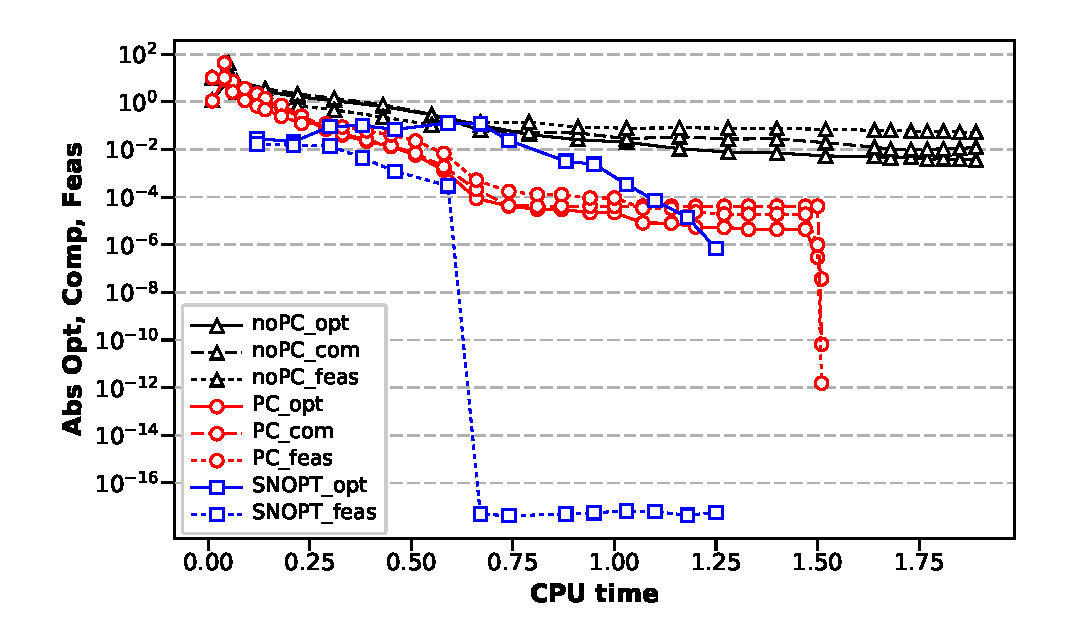
\includegraphics[clip,width=0.7\linewidth]{./figs/newres2/quadratic_200_color.eps} }
   \hspace{1em}
   \subfloat[$n=500$\label{fig:quad_500}]{
   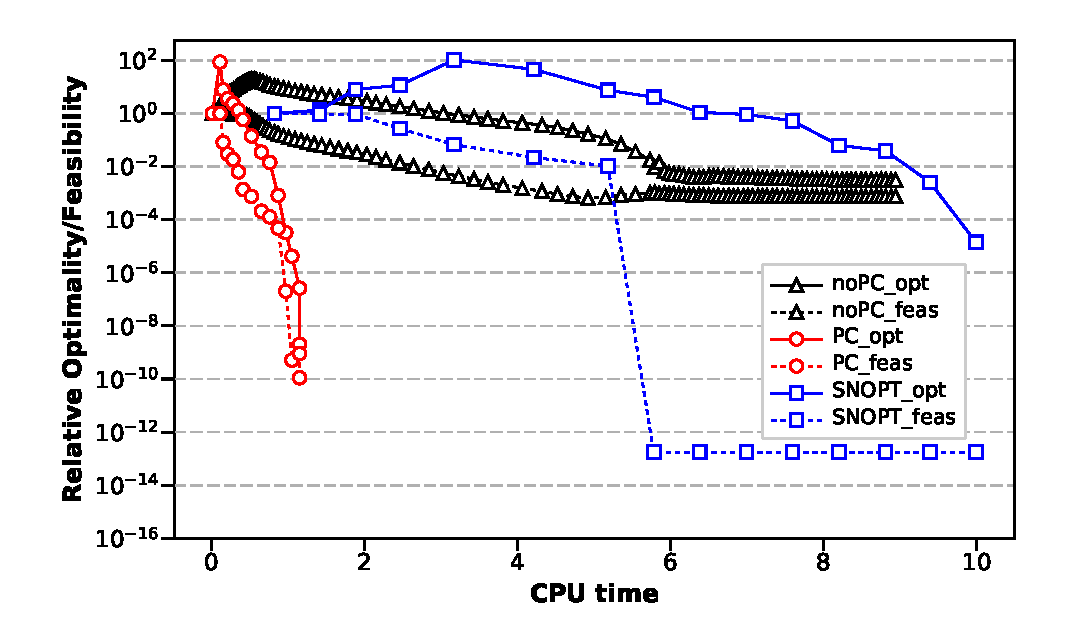
\includegraphics[clip,width=0.7\linewidth]{./figs/newres2/quadratic_500_color.eps} }
   \caption{Convergence histories for the quadratic problem with $n=200$ and
  $n=500$. The results for the proposed algorithm, with and without
  preconditioning, are plotted together with the results from
  SNOPT.\label{fig:quad_hist}}
\end{figure}


To further explore the scalability of the proposed algorithm,
Figure~\ref{fig:quad_scale} plots the total CPU time required by the
preconditioned predictor-corrector algorithm and SNOPT to converge the quadratic
problem as a function of the number of design variables.  For this problem, the
cost of the proposed algorithm grows modestly with $n$ relative to SNOPT.

\begin{figure}[tbp]
  \centering
  \includegraphics[clip,width=0.8\textwidth]{./figs/newres2/quadratic_random_100.eps}%
  \caption{CPU cost versus number of design variables for the quadratic
    optimization problem.\label{fig:quad_scale}}
\end{figure}










